\section{Theorie}
\label{sec:Theorie}

\begin{figure}
    \centering
    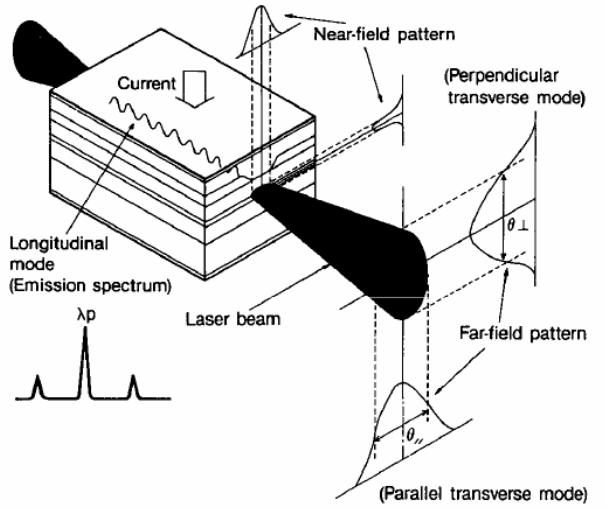
\includegraphics[width=0.8\textwidth]{LaserChip.png}
    \caption{Schematischer Aufbau eines Diodenlaser-Chips \cite{ap60}.}
    \label{fig:LaserChip}
\end{figure}


\begin{figure}
    \centering
    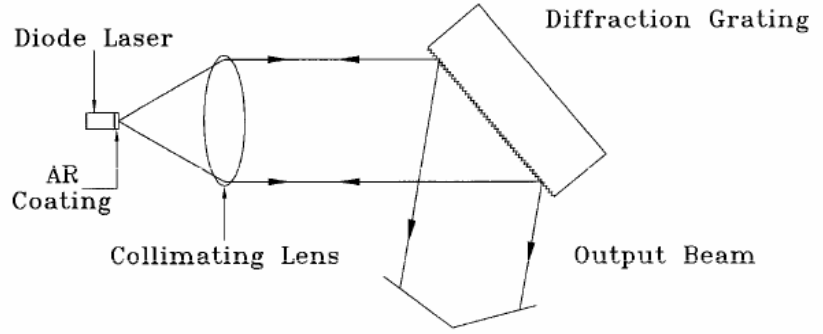
\includegraphics[width=0.8\textwidth]{LittrowSetup.png}
    \caption{Schematischer Aufbau des Laser-Systems (Littrow-Konfiguration) \cite{ap60}.}
    \label{fig:Littrow}
\end{figure}


\begin{figure}
    \centering
    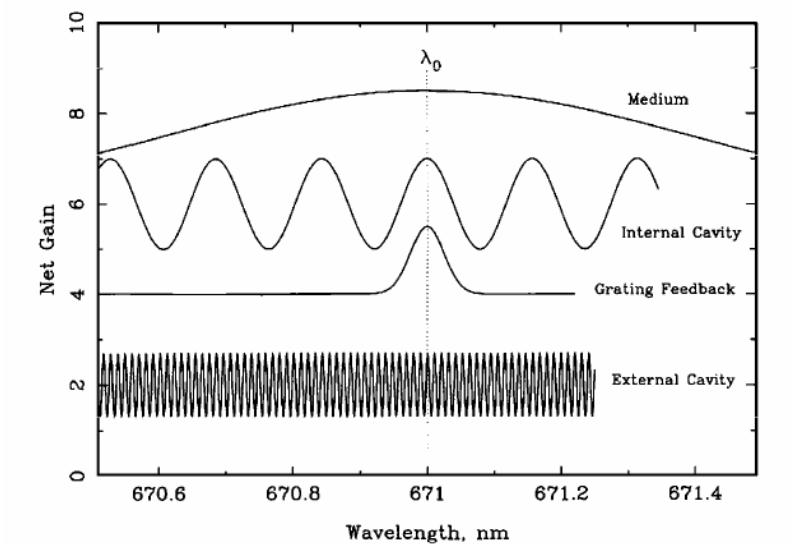
\includegraphics[width=0.8\textwidth]{NetGain.png}
    \caption{Beiträge verschiedener Bauteile zur Verstärkung \cite{ap60}.}
    \label{fig:Gain}
\end{figure}


\begin{figure}
    \centering
    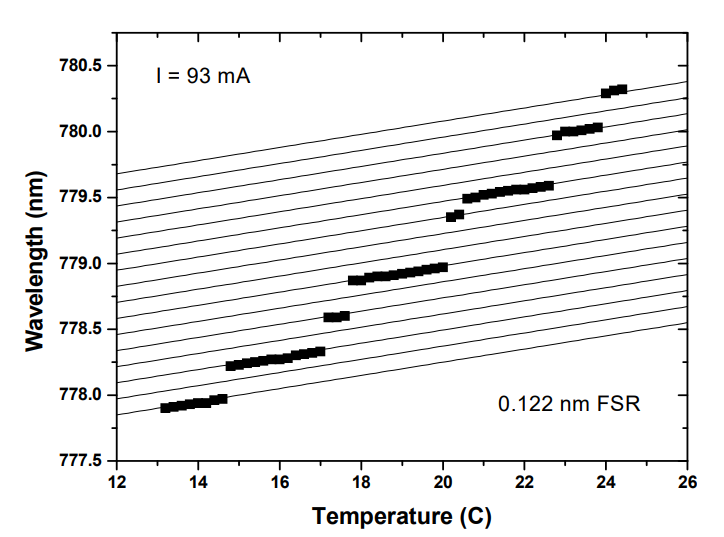
\includegraphics[width=0.8\textwidth]{ModeTemp.png}
    \caption{Einfluss der Temperatur auf das Modenspektrum und die Wellenlänge \cite{ap60}.}
    \label{fig:Temp}
\end{figure}


\begin{figure}
    \centering
    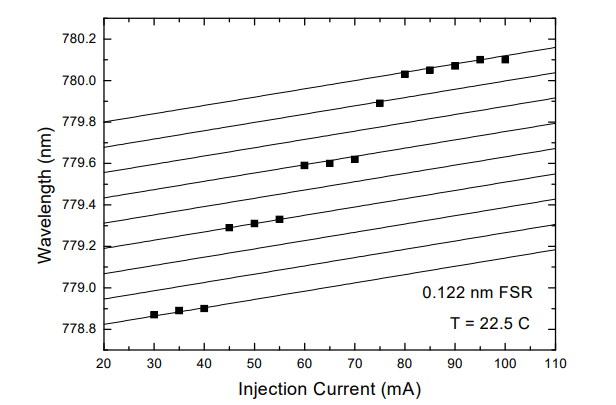
\includegraphics[width=0.8\textwidth]{ModeCurr.png}
    \caption{Einfluss des Pump-Stroms auf die Wellenlänge \cite{ap60}.}
    \label{fig:Curr}
\end{figure}


\begin{figure}
    \centering
    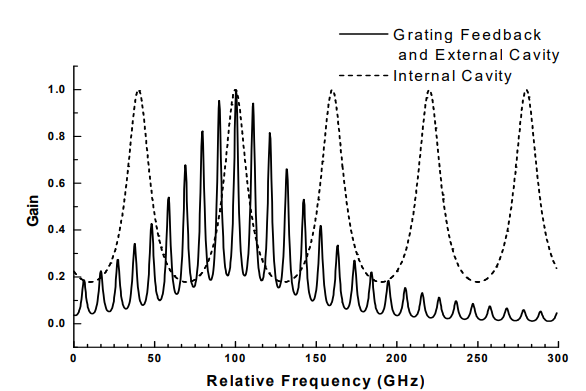
\includegraphics[width=0.8\textwidth]{CavityIdeal.png}
    \caption{Überlagerung des Einflusses des inneren Resonators, des Gitter Feedbacks und des äußeren Resonators \cite{ap60}.}
    \label{fig:GainIdeal}
\end{figure}


\begin{figure}
    \centering
    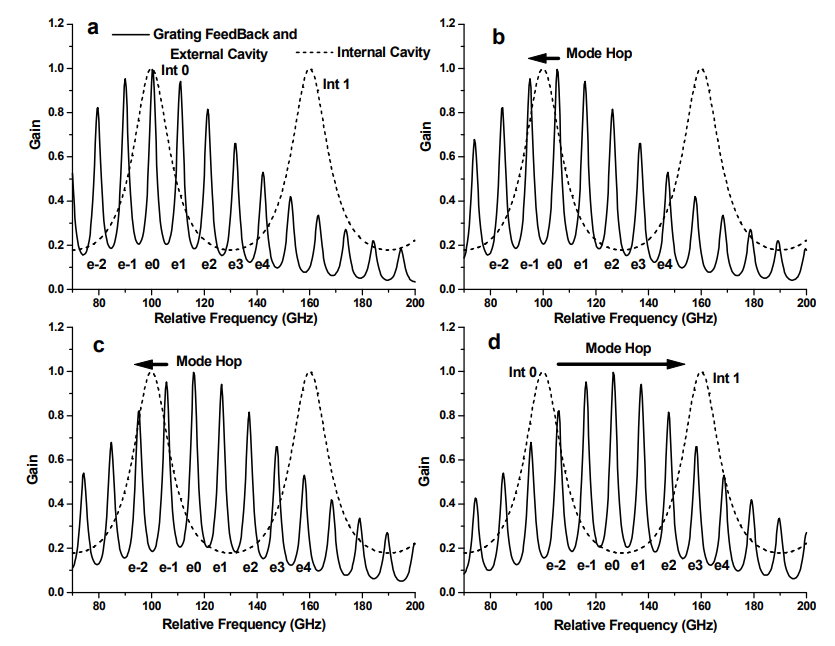
\includegraphics[width=0.8\textwidth]{ModeShifts.png}
    \caption{Einfluss der Justierung des Gitters auf das Modenspektrum \cite{ap60}.}
    \label{fig:ModeShifts}
\end{figure}


\begin{figure}
    \centering
    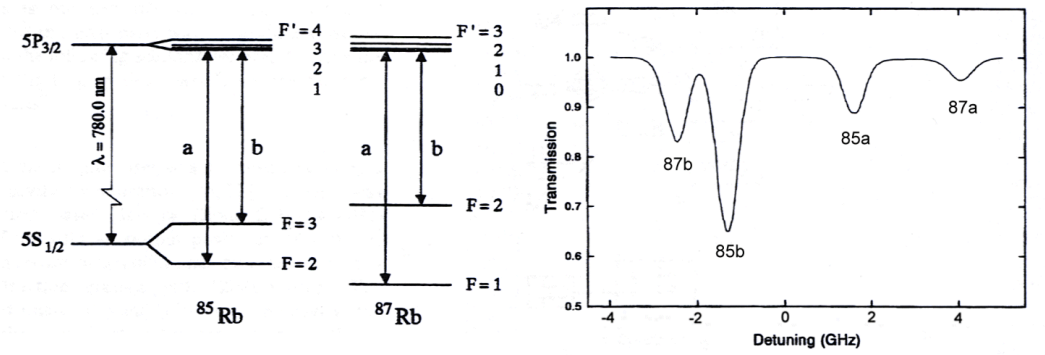
\includegraphics[width=0.9\textwidth]{SpectrumIdeal.png}
    \caption{Spektrum von Rubidium \cite{ap60}.}
    \label{fig:RbSpectrum}
\end{figure}